\chapter{ETL, Metadados e Análise de Dados}
\label{cap:etl-bi}

\section{ETL (Apache Airflow)}
\label{sec:etl}

Duas DAGs, sempre corporativo antes de \textit{marting}:

\begin{itemize}
    \item \textbf{Carga inicial}: lê Northwind/Mercearia direto, popula o corporativo (\textit{upsert} idempotente nas tabelas de apoio) e depois os Data Marts a partir dele; fatos recriados do zero (\texttt{DELETE} + \texttt{INSERT});
    \item \textbf{Carga incremental}: usa o maior id de origem já carregado no corporativo como corte do que é novo; área de \texttt{staging} intermediária (única etapa que lê as origens); atualiza dimensões e insere só as linhas novas nos fatos, sem reler as origens.
\end{itemize}

\section{Catálogo de metadados}
\label{sec:metadados}

Esquema \texttt{metadados}: liga cada campo do DW ao seu campo transacional de origem (ou a um dado externo), com a regra de transformação aplicada. 28 tabelas / 158 campos transacionais, 10 tabelas / 109 campos do DW, 123 linhas de linhagem. DDL completo no \autoref{apend:ddl-metadados}.

\begin{figure}[H]
  \centering
  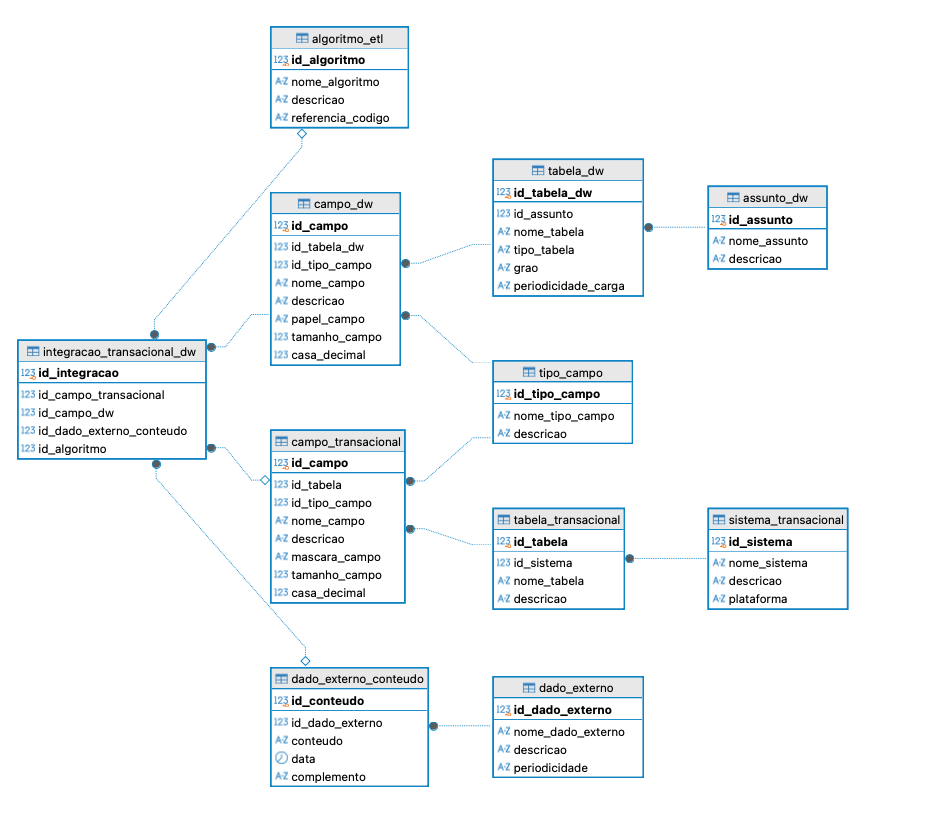
\includegraphics[width=0.9\textwidth]{./fig/metadados_modelo.png}
  \caption{Diagrama entidade-relacionamento do catálogo de metadados}
  \label{fig:metadados-modelo}
  \fontefig{Elaborada pelo autor.}
\end{figure}

\section{Business Intelligence (Metabase)}
\label{sec:bi}

Um painel por Data Mart, com consultas nativas em SQL: \textbf{Vendas} (total, ticket médio, top produtos/clientes, vendas por mês/categoria); \textbf{Compras} (\textit{lead time}, top fornecedores, compras por mês); \textbf{Logística} (prazo médio, atraso por transportadora, \% no prazo).

\begin{figure}[H]
  \centering
  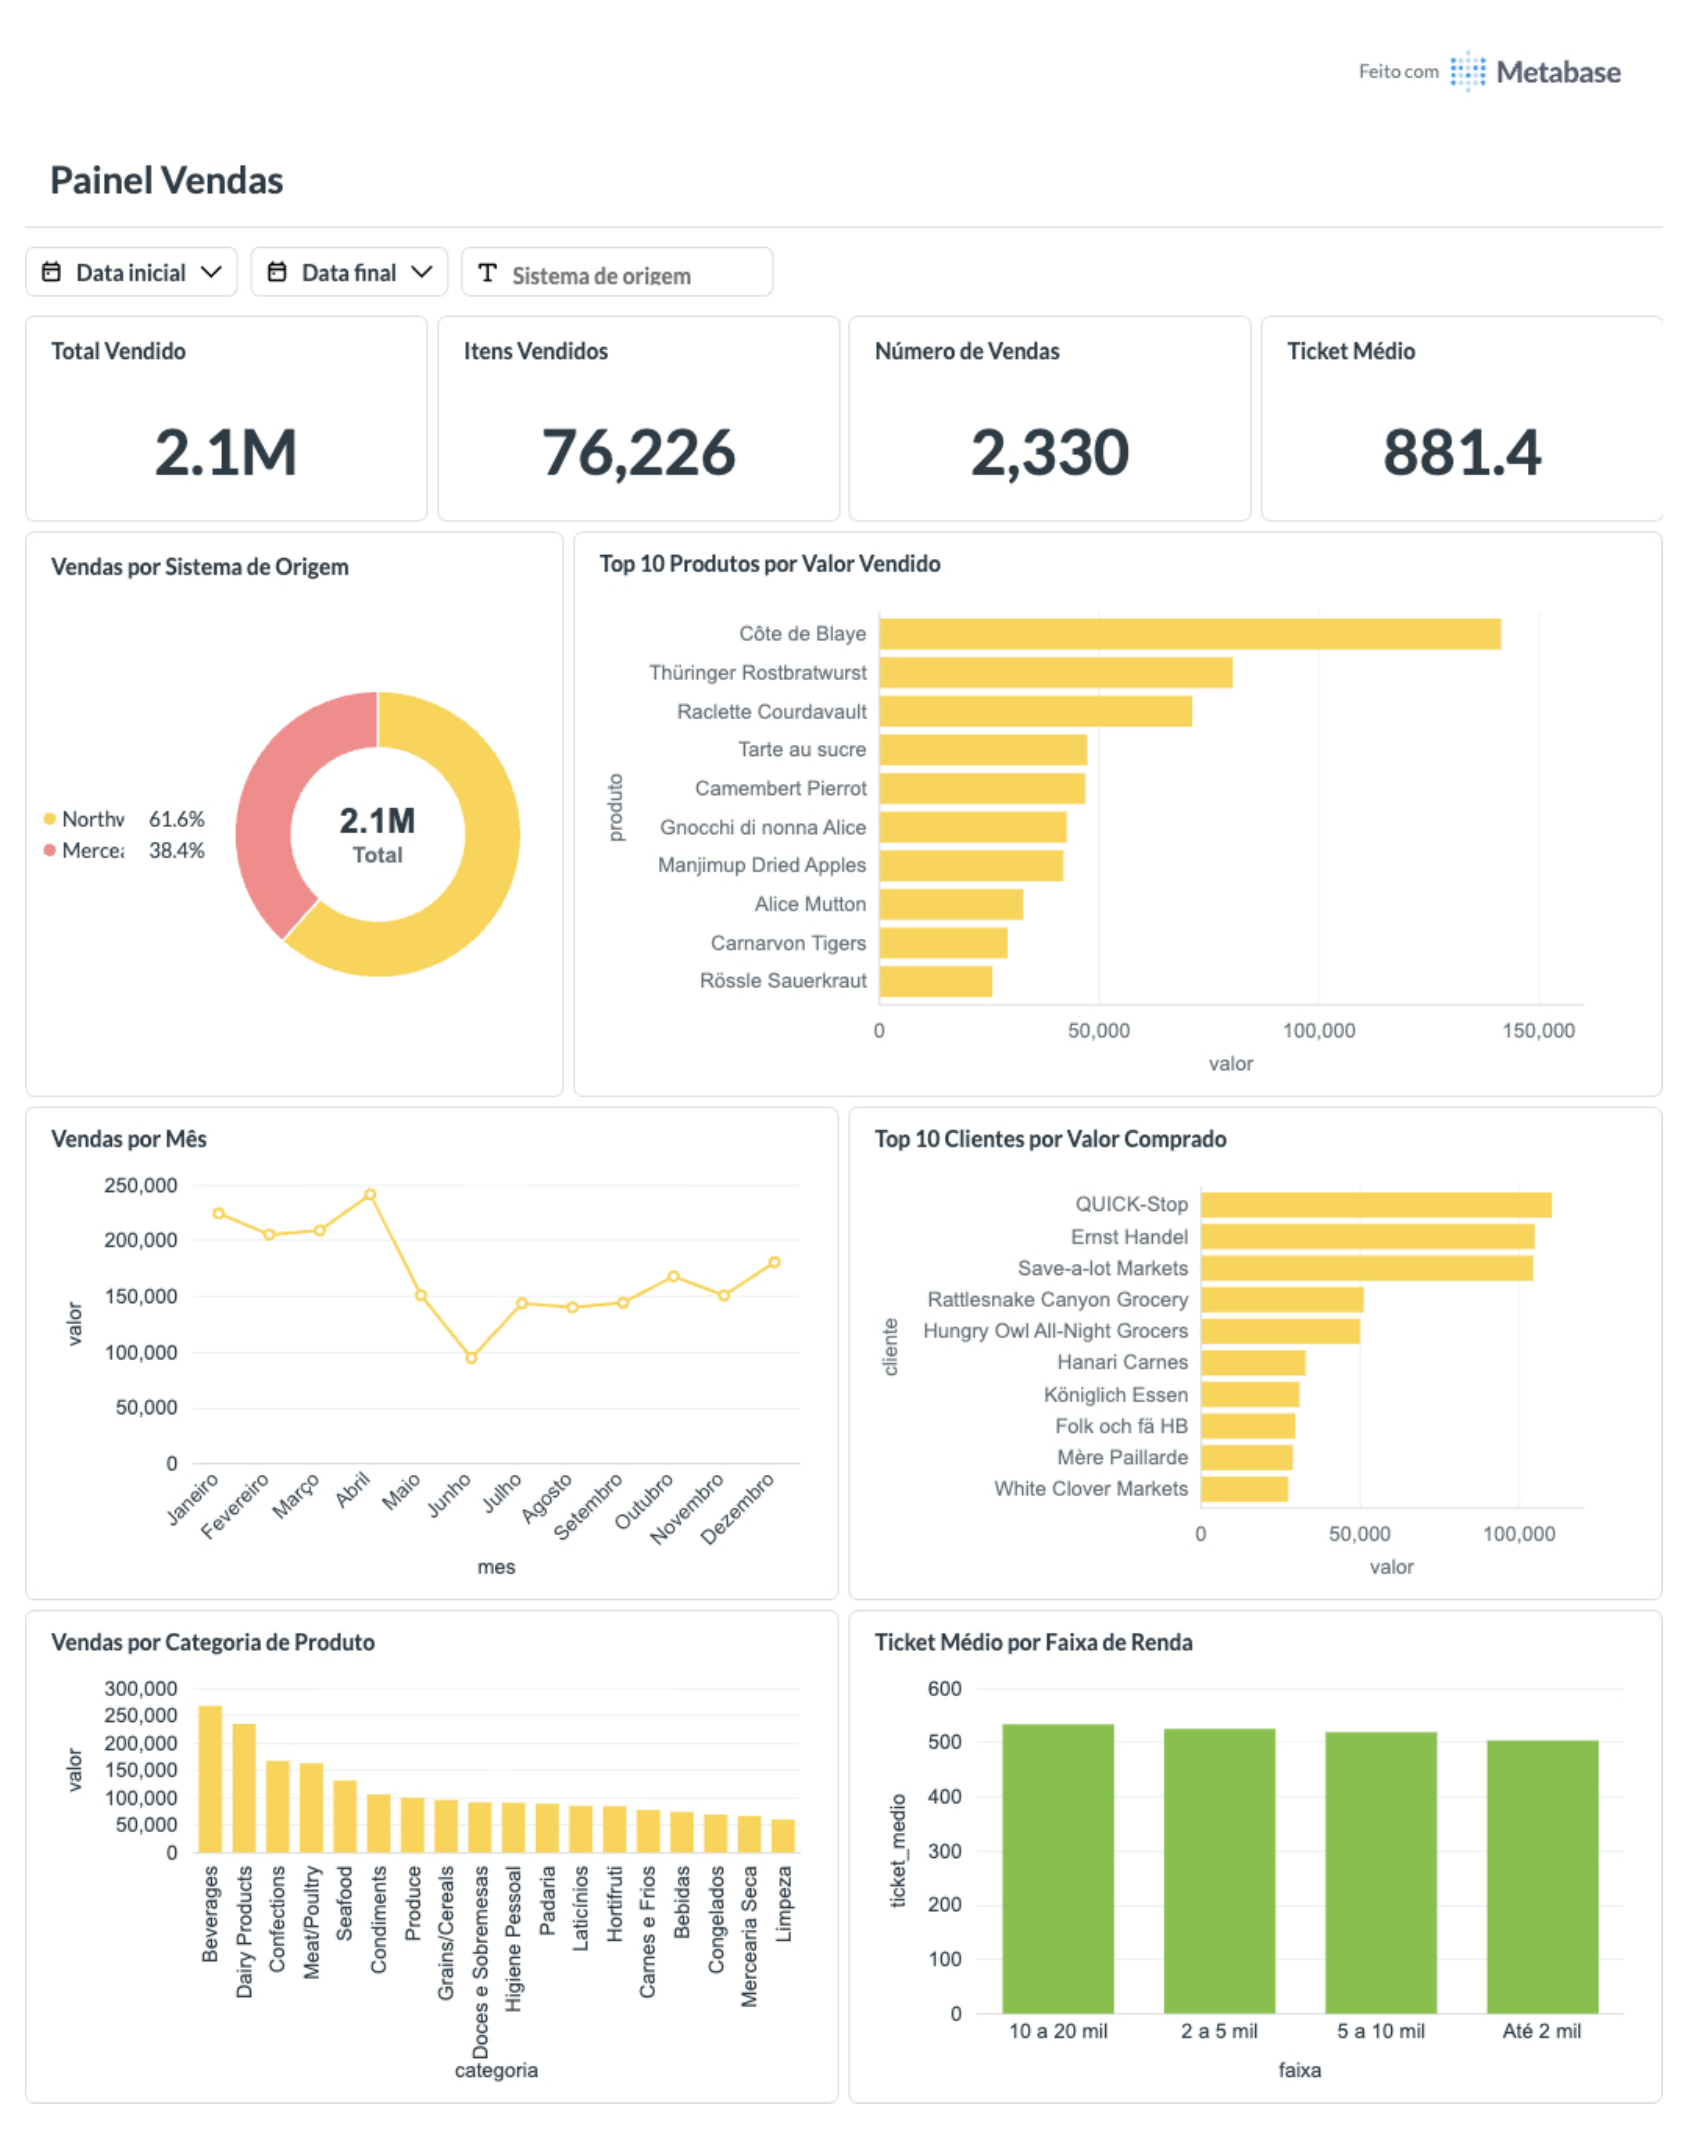
\includegraphics[width=0.75\textwidth]{./fig/dashboard_vendas_preview.png}
  \caption{Painel Vendas no Metabase}
  \label{fig:dashboard-vendas}
  \fontefig{Elaborada pelo autor, a partir do Metabase.}
\end{figure}
